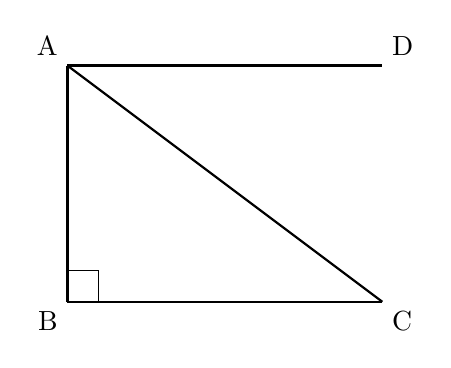
\begin{tikzpicture}

    % Define the coordinates
    \coordinate (A) at (0, 3);       % Top left vertex
    \coordinate (B) at (0, 0);       % Bottom left vertex
    \coordinate (C) at (4, 0);       % Bottom right vertex
    \coordinate (D) at (4, 3);       % Top right vertex
    
    % Draw the quadrilateral ABCD (rectangle outline)
    % Left side AB
    \draw[thick] (A) -- (B);
    
    % Bottom side BC
    \draw[thick] (B) -- (C);
    
    % Top side AD
    \draw[thick] (A) -- (D);
    
    
    % Draw the diagonal AC
    \draw[thick] (A) -- (C);
    
    % Draw the right angle symbol at B
    \draw (0, 0.4) -- (0.4, 0.4) -- (0.4, 0);
    
    % Label point A
    \node[above left] at (A) {A};
    
    % Label point B
    \node[below left] at (B) {B};
    
    % Label point C
    \node[below right] at (C) {C};
    
    % Label point D
    \node[above right] at (D) {D};
    
    \end{tikzpicture}